\section{Definizione del prodotto}

% Nell'indice proposto da Tullio c'è:
% a. Metodo e formalismo di specifica
% b. Presentazione dell'architettura generale del sistema e identificazione dei componenti architetturali di alto livello
\subsection{Formalismo di specifica}

\subsection{Architettura di sistema}

\begin{figure}
\centering
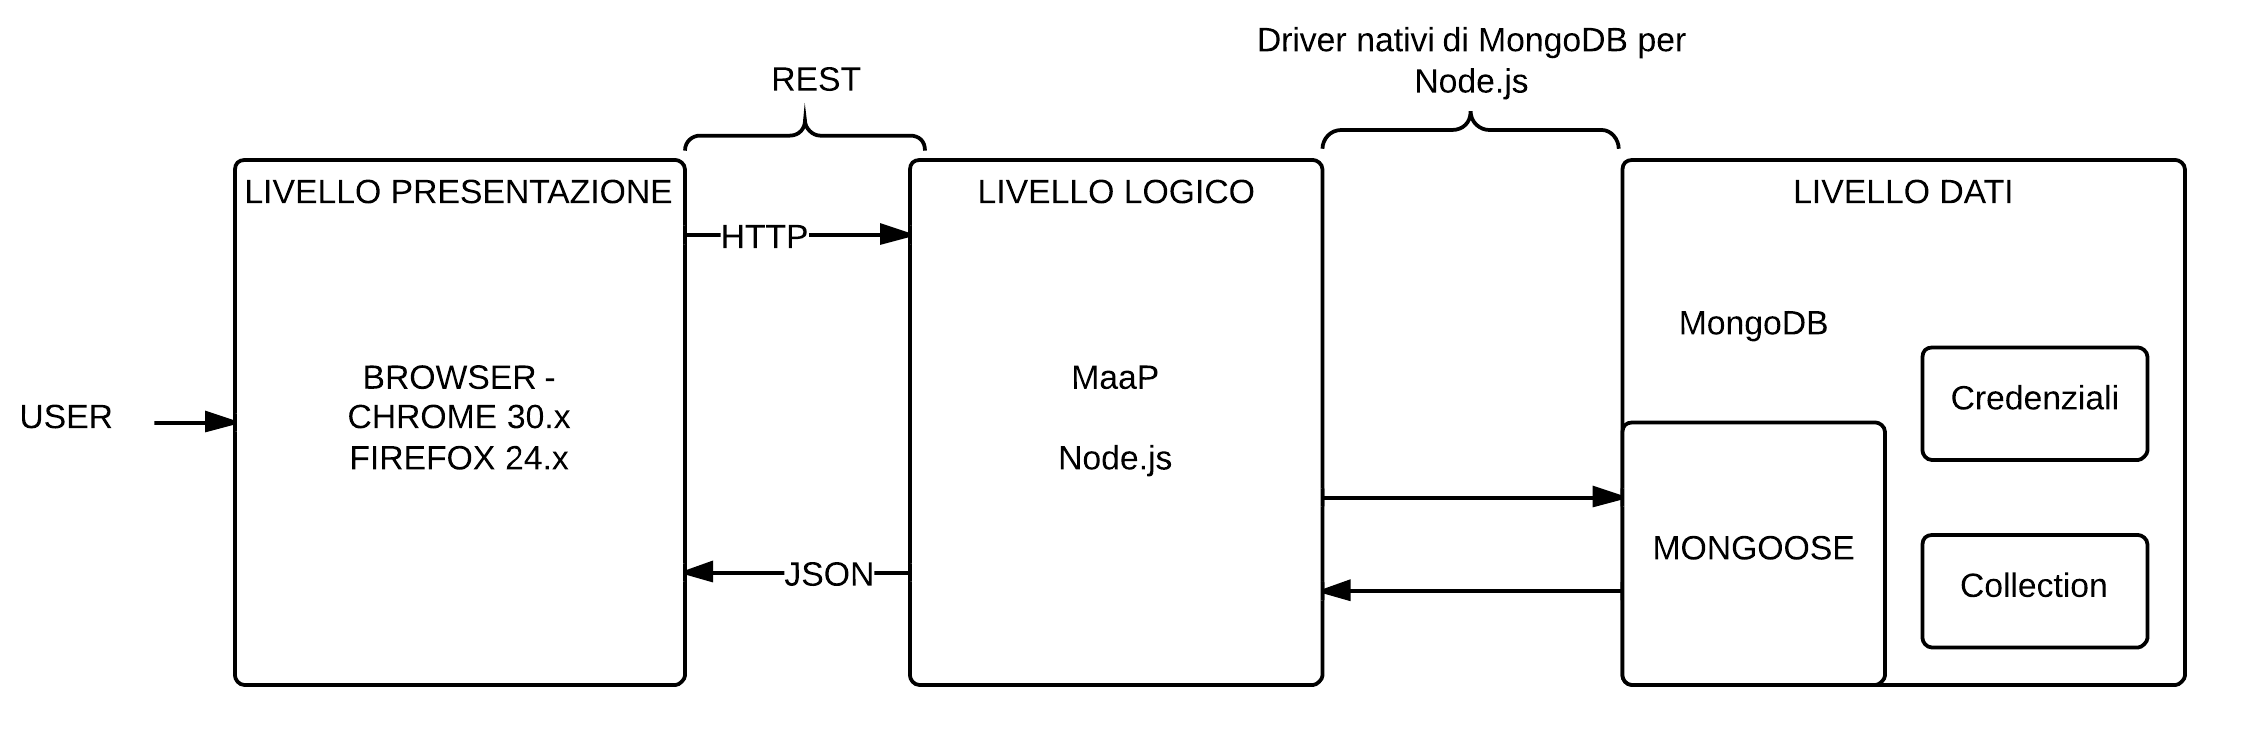
\includegraphics[scale=7]{3-TIER.png}
\caption{Schema del modello utilizzato}\label{fig:1}
\end{figure}

\subsection{Three-Tier Architecture}

Nota: Di seguito i termini modulo, strato e livello sono utilizzati .... 
Si tratta di un architettura di tipo client-server, in cui i processi logici, la persistenza dei dati e l'interfaccia utente sono sviluppati e mantenuti in moduli tra loro indipendenti e distribuiti, il vantaggio che ne consegue è che un modulo può essere aggiornato o sostituito senza dover alterare gli altri.
I tre livelli presenti sono:
\begin{itemize}
\item \textbf{Livello di presentazione} Si tratta dello strato che comunica con l'utente, il quale è estraneo all'esistenza degli altri moduli. Il compito di questo strato è fornire un'interfaccia utente, che comunicherà con il modulo logico per aggiornarsi e trasmettere le scelte dell'utente. Solitamente questo livello si trova sul client.
\item \textbf{Livello logico} Questo livello racchiude le funzionalità, i processi e gli algoritmi dell'applicazione. Solitamente questo livello si trova su un server, e si rapporta con il livello interfaccia e il livello dati. 
\item \textbf{Livello dati} In questo livello solitamente si trovano le \glossario{basi di dati} che garantiscono la persistenza dei dati. E' accessibili solo attraverso il livello logico, che ne garantisce la consistenza. In questo livello si trovano anche i componenti utili all'accesso della base di dati, nel nostro caso \glossario{Mongoose}.
E' importante far notare che uno strato dati può comunicare con più strati logici, che potranno utilizzare i dati in maniera diversa.
\end{itemize}


\subsubsection{REST}

REST, ovvero Representational State Transfer è un tipo di \glossario{RPC}. Si basa su un protocollo di comunicazione \glossario{stateless} di tipo client-server, e solitamente tale protocollo è \glossario{HTTP}, per \ProjectName è invece stato scelto \glossario{HTTPS}.

I motivi che hanno spinto alla scelta di REST sono:
\begin{itemize}
\item Semplicità di utilizzo;
\item Indipendenza dal sistema operativo utilizzato dal client;
\item Indipendente dai linguaggi di programmazione utilizzati;
\item In coppia con HTTPS permette una certa sicurezza delle comunicazioni.
\end{itemize}

REST utilizza il concetto di risorsa, ovvero un aggregato di dati con un nome (\glossario{URI}) e una rappresentazione, su cui è possibile invocare le operazioni \glossario{CRUD} tramite il protocollo sopracitato.

Nell'URL inviato sono presenti il nome della risorsa e la sua rappresentazione, identificata dall'estensione del file scelta, e per \ProjectName è stato scelto il formato \glossario{JSON}, in quanto il suo parsing in \glossario{JavaScript} è più semplice rispetto, ad esempio, quello di \glossario{XML} o \glossario{CSV}.

Un'altra caratteristica di REST è che essendo \glossario{stateless} ogni richiesta dovrà contenere tutte le informazioni necessarie, e non dipende dallo stato del sistema.